% Chapter 1

\chapter{Introducción General} % Main chapter title

\label{Chapter1} % For referencing the chapter elsewhere, use \ref{Chapter1} 
\label{IntroGeneral}

%----------------------------------------------------------------------------------------

% Define some commands to keep the formatting separated from the content 
\newcommand{\keyword}[1]{\textbf{#1}}
\newcommand{\tabhead}[1]{\textbf{#1}}
\newcommand{\code}[1]{\texttt{#1}}
\newcommand{\file}[1]{\texttt{\bfseries#1}}
\newcommand{\option}[1]{\texttt{\itshape#1}}
\newcommand{\grados}{$^{\circ}$}

%----------------------------------------------------------------------------------------

En este capítulo se presentan el contexto del proyecto, los sistemas ferroviarios, una introducción a las distintas tecnologías de los sistemas de enclavamientos y los objetivos a cumplir.

%----------------------------------------------------------------------------------------
		
	\section{Contexto y motivación}
	
		Actualmente el sistema ferroviario argentino se encuentra enormemente deteriorado y desactualizado. Mientras que otras naciones mas avanzadas han progresado en la migración de sus sistemas de transporte de cargas y pasajeros añadiendo electrónica de última generación, Argentina continua utilizando mecanismos diseñados a principios o mediados del siglo XX.
		
		%Así, en muchos ferrocarriles, no hay sistemas de seguridad para pasajeros, conductores, peatones y automovilistas. En otras líneas se siguen usando tecnologías de hace más de 50 años, que en los países con alto desarrollo tecnológico han sido reemplazadas hace mucho tiempo\citep{LIBRO1}.
		
		Esto repercute negativamente en la poca o nula seguridad que dichos sistemas pueden brindar a los pasajeros, conductores, peatones y automovilistas. Pero los sistemas electrónicos para la seguridad vial de trenes y subtes son importados y muy costosos, además de estar monopolizados por menos de un docena de empresas en todo el mundo. Un sistema de enclavamiento como el que se aborda en este trabajo puede costar entre 5 y 10 millones de dólares\citep{SIEMENS} y se requieren varias decenas de estos sistemas sólo para la zona urbana de la Ciudad Autónoma de Buenos Aires.
		
		Dichas empresas brindan muy poca información técnica sobre sus desarrollos y la mayoría de las herramientas que utilizan son de uso privado empresarial. No obstante, deben regirse bajo normativas como las que la comunidad europea ha establecido desde 2004. Normas ferroviarias relacionadas con los parámetros RAMS, haciendo especial hincapié en la seguridad. En este sentido, las tres normas principales son EN-50126\citep{EN50126} (ciclo de vida), EN-50128\citep{EN50128} (técnicas de software) y EN-50129\citep{EN50129} (técnicas de hardware). Entre otras cuestiones, se busca asegurar la integridad de la seguridad.	
		
		En los sistemas críticos una falla puede poner en peligro cientos de vidas humanas y/o costosas inversiones. Por lo tanto se deben cumplir estrictos parámetros de fiabilidad, disponibilidad, mantenibilidad y seguridad (RAMS, del inglés \textit{Reliability}, \textit{Availability}, \textit{Mantenibility} \textit{and} \textit{Safety}), durante todo el ciclo de vida.
		
		En este contexto en 2015 se crea el CONICET-GICSAFe, cuyas siglas corresponden a Grupo de Investigación en Calidad y Seguridad de las Aplicaciones Ferroviarias, conformado por docentes e investigadores de una decena de universidades e instituciones públicas argentinas\citep{GICSAFE}. El grupo desarrolla sistemas electrónicos e informáticos para aplicaciones ferroviarias relacionadas con la seguridad, generando un prototipo funcional y la documentación correspondiente que luego se transfiere en su totalidad a los clientes. En particular, esta metodología se utiliza en este trabajo con Trenes Argentinos, que es la Sociedad del Estado que opera las líneas Roca, Sarmiento, Mitre, San Martin y Belgrano Sur, entre otras. Luego el cliente puede fabricar el sistema diseñado por el GICSAFe o licitar su fabricación, así como modificar el sistema de acuerdo con sus necesidades.   
	
		En el marco de la Especialización de Sistemas Embebidos, desde julio de 2018 se tuvieron reuniones con diferentes funcionarios y profesionales de Trenes Argentinos. En particular los encuentros se desarrollaron con la Gerencia de Ingeniería, Gerencia de Seguridad Operacional, Subgerencia de Desarrollo y Normas Técnicas, Subgerencia de Transporte, Gerencia de Señalamiento, entre otros, de los cuales surgió el interés en el desarrollo del presente proyecto. De dichas visitas y otras posteriores se obtienen la totalidad de las fotografías incluidas en esta memoria.
			 	
		El desarrollo del sistema implica muchas áreas distintas a tener en cuenta: procesamiento, comunicación, replicación del sistema para otras topologías, testing, etc. Un primer prototipo se desarrolló a finales de 2018 y actualmente se culminó una segunda versión para la Maestría en Sistemas Embebidos. Sin contar que la amplia variedad de topologías existentes obliga a abandonar la metodología de desarrollo artesanal de cada sistema y abordarlo de forma general para topologías genéricas, lo que adiciona aún mas trabajo al monumental proyecto.		
		
		Por esa razón, durante la Maestría en Sistemas Embebidos, en el año 2019, se comenzó a seguir un estrategia orientada a obtener una solución integral para cualquiera sea la locación, generando automáticamente el código y los testbenchs involucrados. A la vez que miembros de CONICET-GICSAFe pertenecientes a UTN-Haedo comenzaron el desarrollo de un front-end gráfico y su correspondiente simulador en tiempo real, en vistas a ser integrado al proyecto en el mediano plazo.
	
		Hacia finales del 2019 se iniciaron reuniones con miembros de la Comisión Nacional de Energía Atómica(CNEA), para integrar el proyecto en sus plataformas de hardware ampliamente testeadas en el ámbito de los sistemas críticos. Además del intercambio de conocimiento y la puesta en común de estrategias a utilizar, se aprovechó todo lo posible la amplia experiencia que ellos nos brindaron durante el pasado y corriente año.
		
	\section{Propuesta de solución}	
		
		En el desarrollo del proyecto en la Especialización de Sistemas Embebidos se implementaron sistemas como el de la Figura \ref{fig:CESE_1}. Con una cantidad acotada de tramos de vías y bifurcaciones que implicaba una cantidad acotada de circuitos lógicos complicados pero posibles de obtener y testear.
		
		La implementación del sistema se hacía de forma artesanal, bloque a bloque y conectándolos de igual manera uno por uno. El testing demoraba días o semanas en estar completo para ser utilizado y era necesario revisar varias veces las pocas y difusas especificaciones que se tenían para corroborar un correcto funcionamiento del sistema.	
		
		\begin{figure}[htbp!]
			\centering
			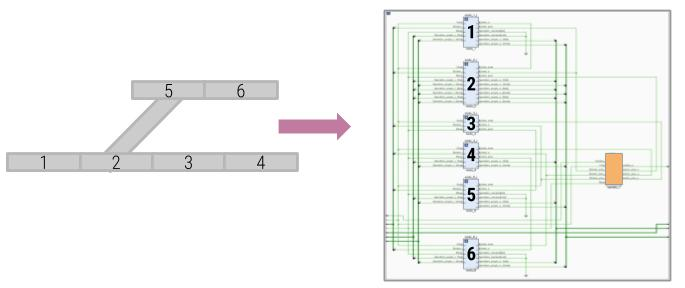
\includegraphics[scale=.5]{./Figures/Grafo_VHDL}
			\caption{Ejemplo de implementación de topología sencilla}
			\label{fig:CESE_1}
		\end{figure}	
		
		\vspace{5cm}
		
		Pero fue una constante que la locación en la cual se basaba el desarrollo del sistema cambiase abruptamente por otra diferente, representada en la Figura \ref{fig:CESE_2}. Por lo que, aún manteniendo los mismos conceptos iniciales, el alcance y los requerimientos cambiaban completamente y se tenía que desechar gran parte de lo construido, tanto del sistema como los tests que ya no tenían sentido para el nuevo sistema. El rediseñar de cero todo fue algo común durante esta etapa del proyecto.
		
		\begin{figure}[htbp!]
			\centering
			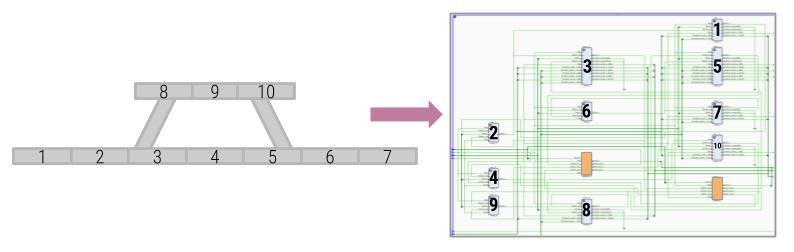
\includegraphics[scale=.5]{./Figures/Grafo_VHDL_B}
			\caption{Ejemplo de implementación de topología compleja}
			\label{fig:CESE_2}
		\end{figure}
			
		Una mayor cantidad de elementos ferroviarios implica una densidad mayor de circuitos lógicos y estos a su vez repercuten en un crecimiento exponencial de la complejidad del desarrollo, mayor dificultad para implementar los ensayos y mayores chances de errores al extrapolar conceptos aún inmaduros a sistemas de mayor tamaño.
		
		La solución a proponer no podía quedar sujeta a una única topología, ya que aún culminando el proyecto se corría el riesgo de que el tiempo empleado fuese desperdiciado si se cambiaban los requerimientos de forma tan abrupta. Es por eso que se añadió como objetivo de este trabajo el desarrollo de una herramienta capaz de generar automáticamente la solución electrónica de un sistema de enclavamiento ferroviario, a partir de una representación matemática única de cada topología. En la Figura \ref{fig:Generacion} se puede visualizar el proceso.
		
		\begin{figure}[htbp!]
			\centering
			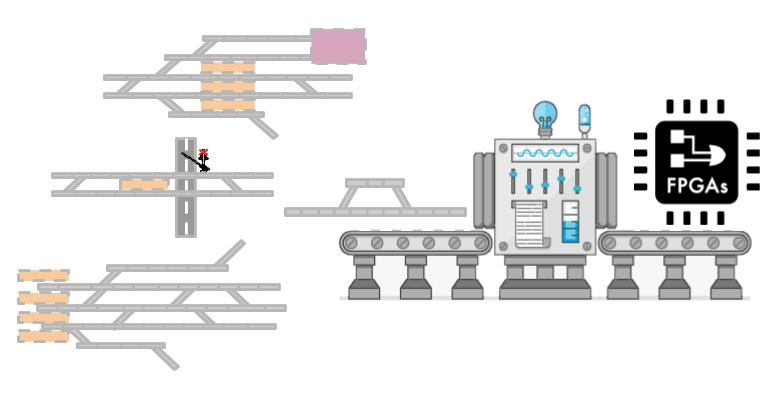
\includegraphics[scale=.5]{./Figures/Generacion}
			\caption{Proceso de generación automática de la solución electrónica}
			\label{fig:Generacion}
		\end{figure}
		
		De esta manera, la solución desarrollada parte de cualquier red ferroviaria, representada mediante un grafo y un analizador de redes ferroviarias (desarrollado también en este trabajo) detecta qué función cumplirá cada elemento de la red y determina cuántos semáforos, de cuantos aspectos, en que orientación y en qué nodo deben situarse para que el sistema sea seguro. A continuación, en base a los semáforos insertados el analizador calcula todas las rutas posibles que admite esa red.
	
		Para poder entender mejor el funcionamiento del sistema es necesario introducir conceptos propios del sistema ferroviario y sus componentes involucrados, que se describirán en la sección siguiente.

	\section{Elementos del sistema ferroviario}
	
		Se denomina señalamiento ferroviario al sistema cuya función es evitar las colisiones entre trenes. A continuación se presentan distintos elementos del señalamiento ferroviario que fueron utilizados durante este trabajo.
		
		\subsection{Vías}
			
			En la Figura \ref{fig:Via_eclisa} se visualiza un tramo de vía ferroviaria. Las vías se separan en tramos y por seguridad se establece que cada tramo de vías puede contener solo una formación por vez. Estos tramos en zonas urbanas tienen una extensión típica de entre 500 y 1000 metros.
			
			\begin{figure}[htbp!]
				\centering
				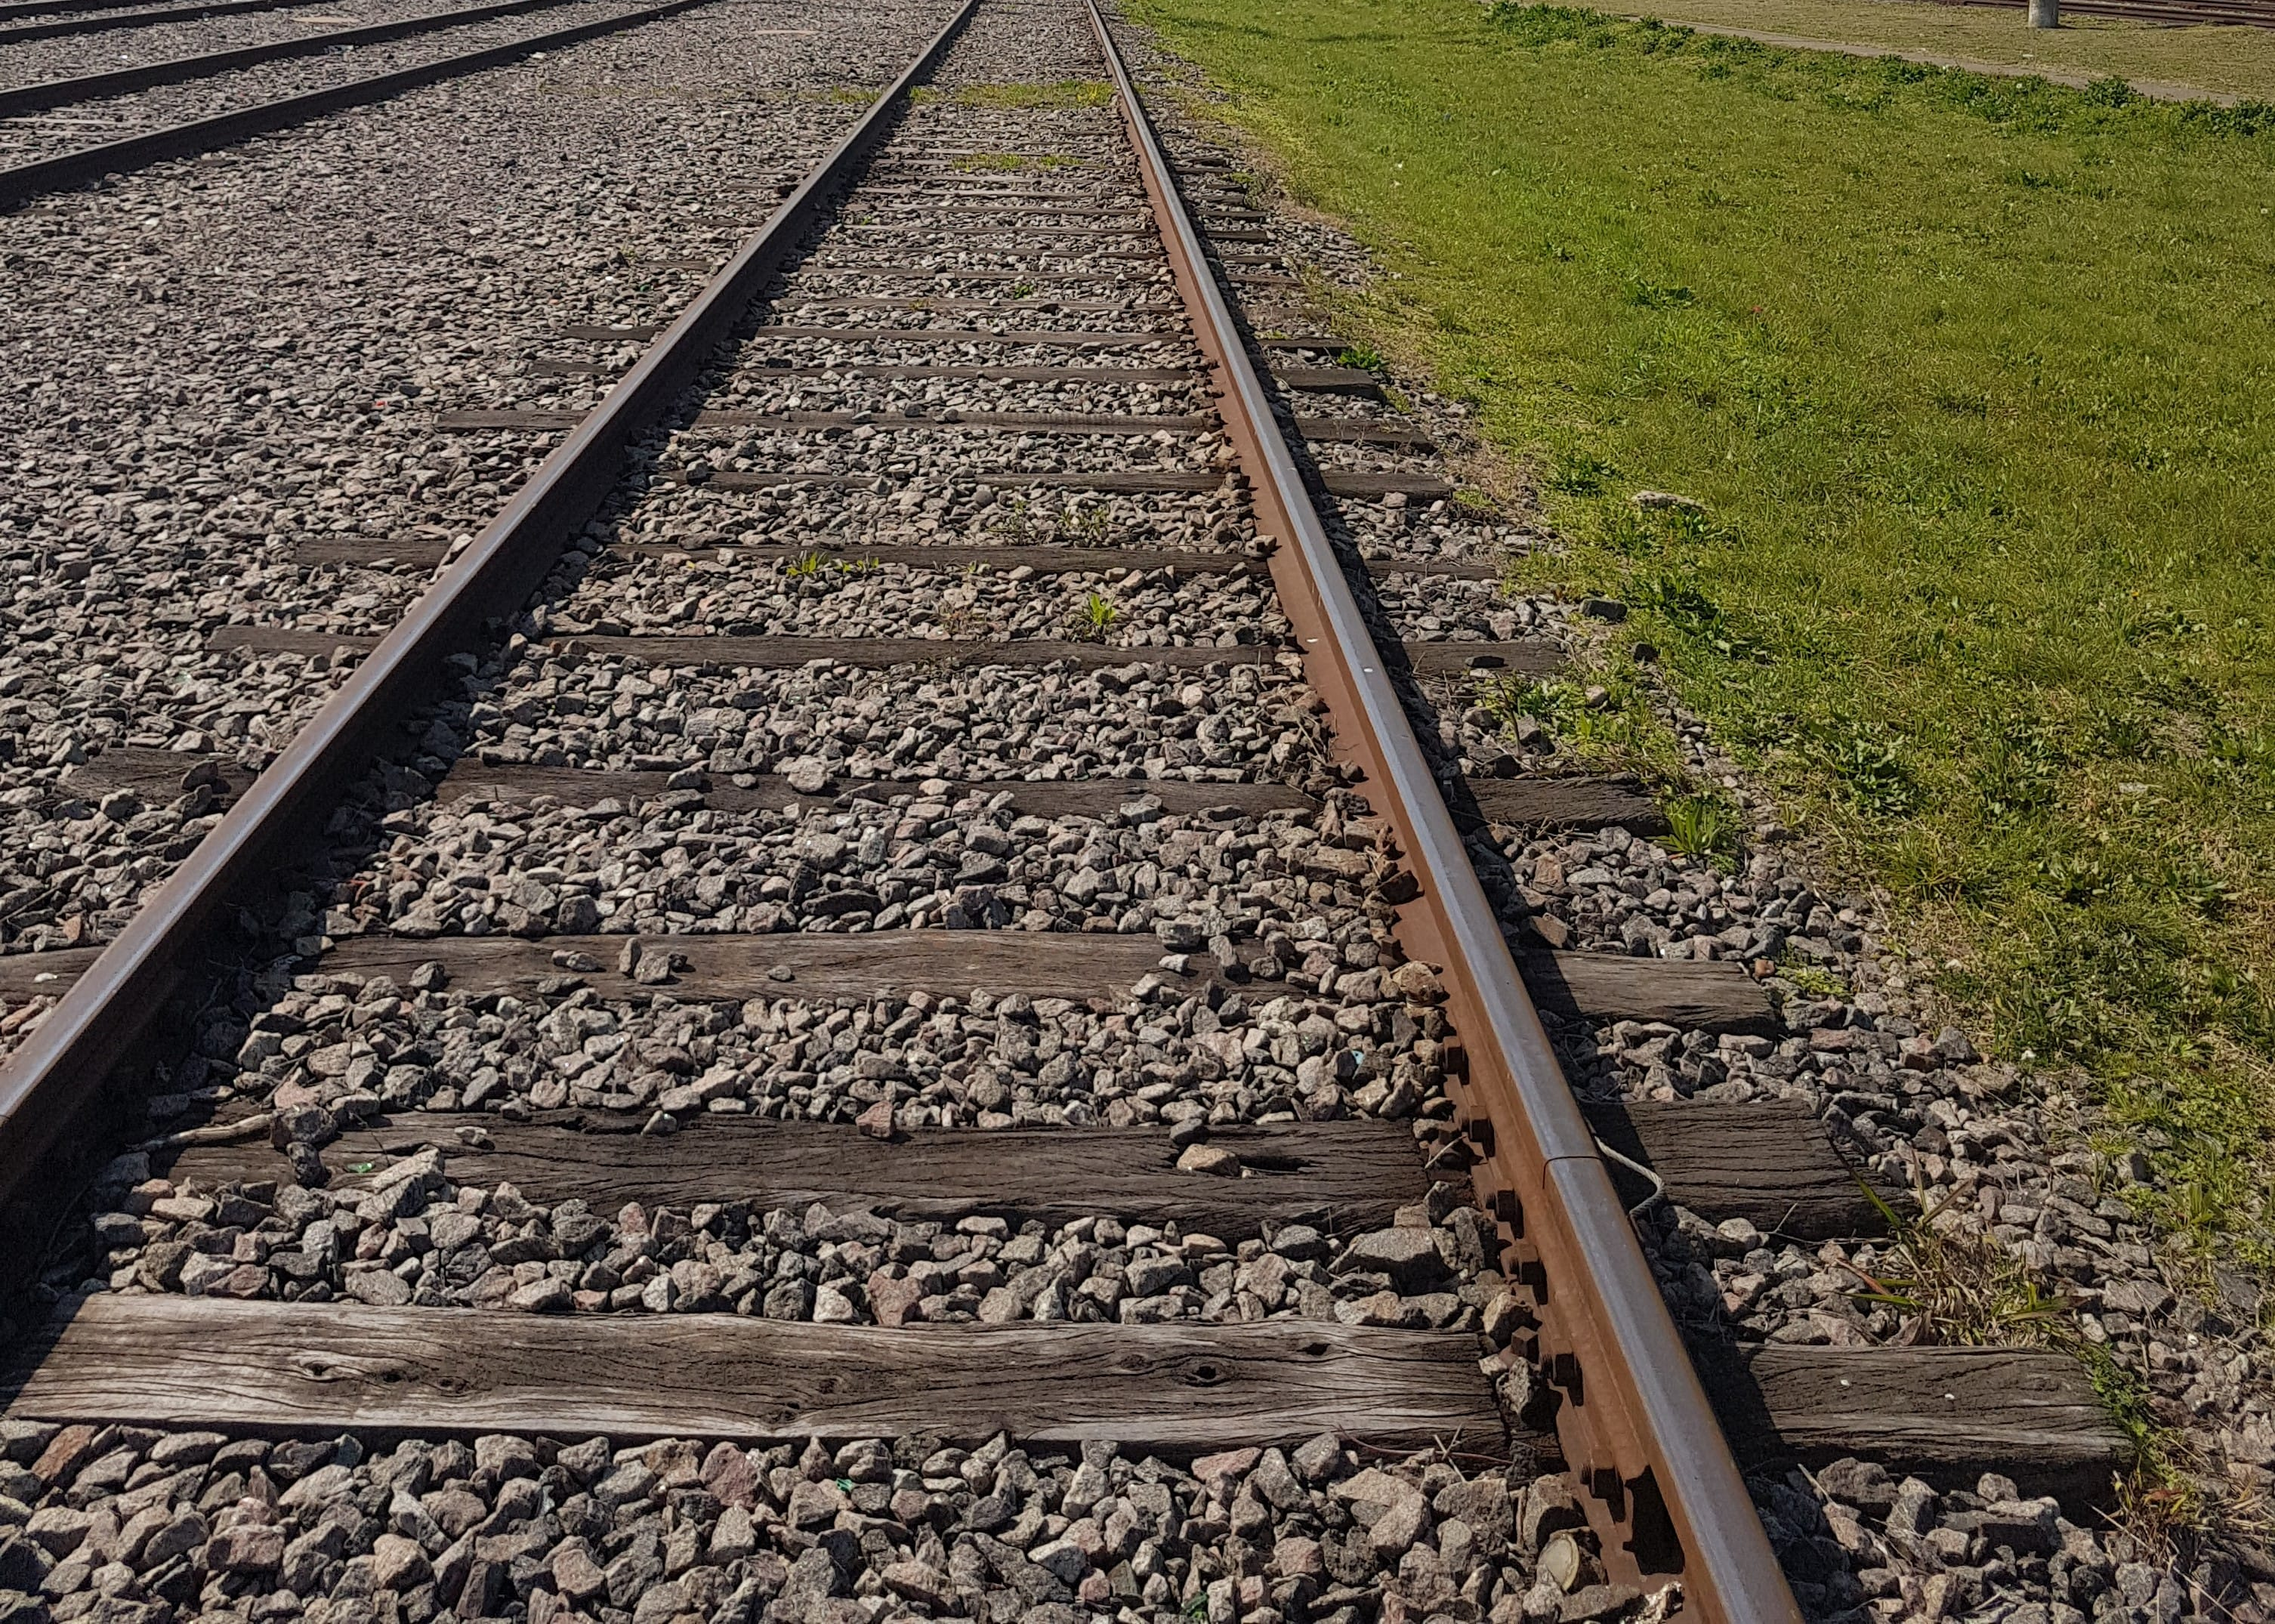
\includegraphics[scale=.12]{./Figures/Tramo_via}
				\caption{Tramo de vía ferroviaria.}
				\label{fig:Via_eclisa}
			\end{figure}					
			
			Las vías pueden ser ascendentes o descendentes. Las ascendentes son aquellas por las que los trenes circulan únicamente en la dirección del kilometraje en sentido creciente. Las descendentes son aquellas por la que los trenes circulan únicamente en la dirección del kilometraje en sentido decreciente\citep{RITO}. Usualmente el kilómetro 0 es la estación principal de la línea ferroviaria, como por ejemplo: Plaza Constitución (para la línea Roca), Once de septiembre (para la línea Sarmiento) o Retiro (para las líneas Mitre y San Martín).
		
			También existen vías simples, banalizadas o de maniobra en las que los trenes pueden circular en ambas direcciones. En este trabajo no se abordarán este tipo de vías, salvo por un pequeño tramo de unos 30 metros en los que se produce el cambio de vía, lo que permite a los trenes pasar de la vía ascendente a la descendente o viceversa.
			
		\subsection{Semáforos ferroviarios}
			
			Los semáforos ferroviarios poseen varias luces, que al encenderse configuran diversos aspectos, cada uno de los cuales posee diferente significado.
			
			La función principal de los semáforos es indicar al conductor ferroviario el tipo de marcha que debe adoptar en el tramo de vía en el que va a ingresar.
			
			A diferencia de los semáforos viales que funcionan con un temporizador, los semáforos ferroviarios cambian su estado en función de la ausencia o presencia de formaciones ferroviarias ocupando vías cercanas, o por la petición de rutas por parte de un operador autorizado.
			
			En la Figura \ref{fig:Sem_3Aspectos} se presenta un esquema de señales de tres aspectos, que es el tipo de semáforo que se utiliza en la gran mayoría de las líneas ferroviarias.
						 	
			 \begin{figure}[htbp!]
				\centering
				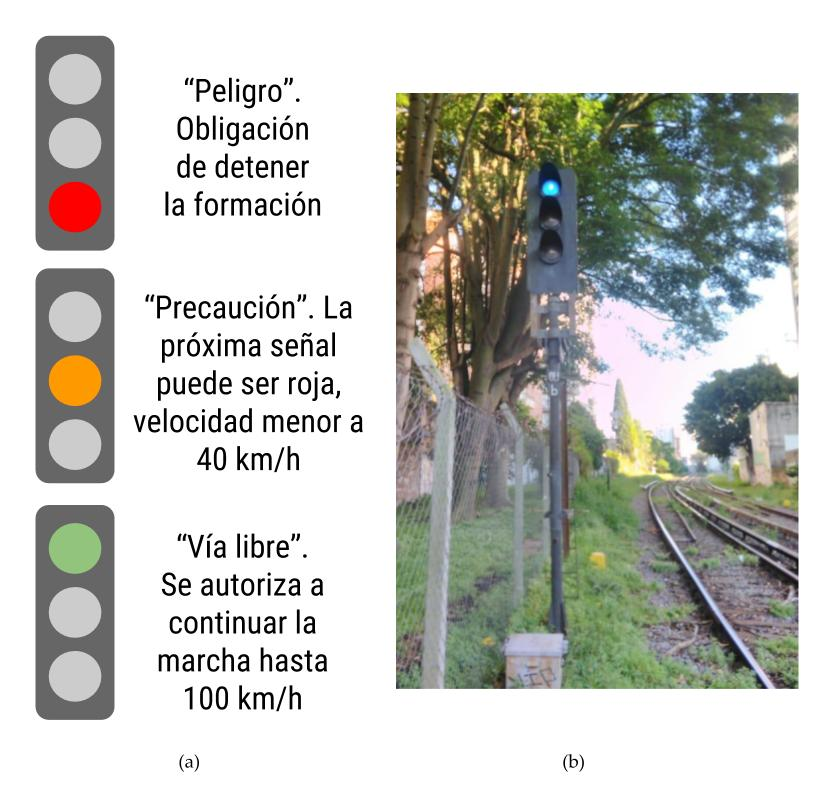
\includegraphics[scale=.33]{./Figures/Sem3}
				\caption{(a) Semáforo de 3 aspectos\\(b) Semáforo doble de 3 aspectos (Estación Olivos).}
				\label{fig:Sem_3Aspectos}
			\end{figure}
	
			%\vspace{5cm}
			
			Los semáforos de dos aspectos, como el que se se visualiza en la Figura \ref{fig:Sem_2Aspectos}, se utilizan en cambios de vías donde por su peligrosidad no se podría permitir un aspecto verde que habilite una velocidad alta. 		
			 
			 \begin{figure}[htbp!]
				\centering
				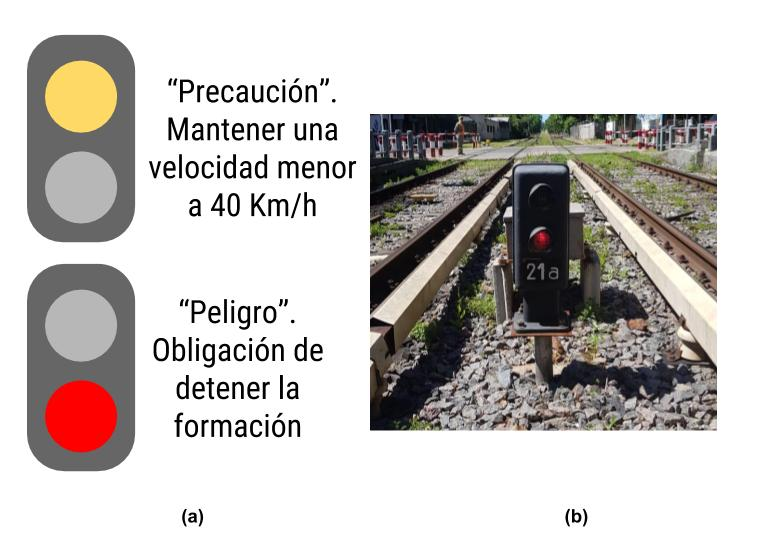
\includegraphics[scale=.35]{./Figures/Sem2}
				\caption{(a) Semáforo de 2 aspectos\\(b) Semáforos de cruce de vías (Estación Lavallol).}
				\label{fig:Sem_2Aspectos}
			\end{figure}				
			
			Los semáforos de cuatro aspectos son utilizados en la Línea Roca y poseen un doble amarillo antes del amarillo simple, para permitir así tramos de vías mas cortos en forma segura. Como no son objeto de estudio del presente trabajo, no serán explicados en esta memoria.
		
		\subsection{Circuito de vías}
		%\label{sec:DOBLE}
			Un circuito de vía es un sistema eléctrico que determina si un tramo de la vía se encuentra ocupado o libre. Se ilustra en la Figura \ref{fig:Ocupacion} que cada tren provoca un cortocircuito en el tramo de vía en que se encuentra, modelado como un 0, y cada ausencia de tren es modelada como un 1.
			
			\begin{figure}[h]
				\centering
				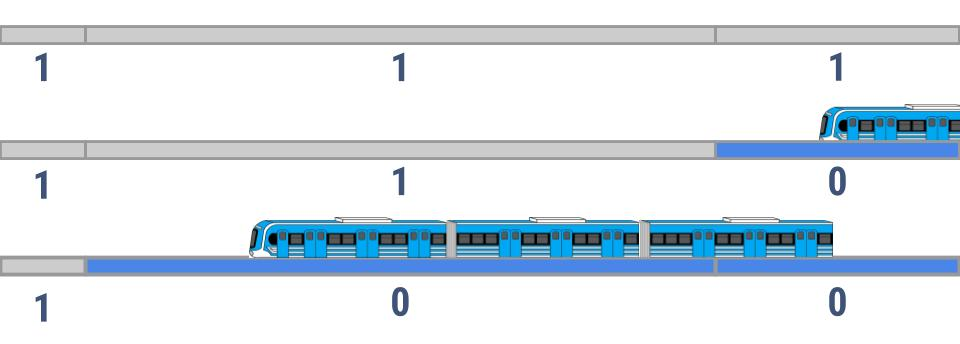
\includegraphics[scale=.4]{./Figures/Ocupacion}
				\caption{Ocupación de las secciones de vías.}
				\label{fig:Ocupacion}
			\end{figure}
			\change{Incluir el tren recortado?}
			
			Dicha ocupación repercute directamente sobre el señalamiento lumínico: si el tramo de vía no tiene ninguna formación ocupándolo, el señalamiento indicará un aspecto verde o amarillo según el estado de ocupación del tramo siguiente, como se ilustra en la Figura \ref{fig:Recubrimiento}.
			
			Si la formación ocupa la sección, el señalamiento cambiará su aspecto a rojo para indicar que no puede ingresar ninguna otra formación, a fin de evitar colisiones. Por seguridad también se establecerá a rojo el semáforo anterior y a amarillo el anterior a éste (doble recubrimiento).
			
			\begin{figure}[h]
				\centering
				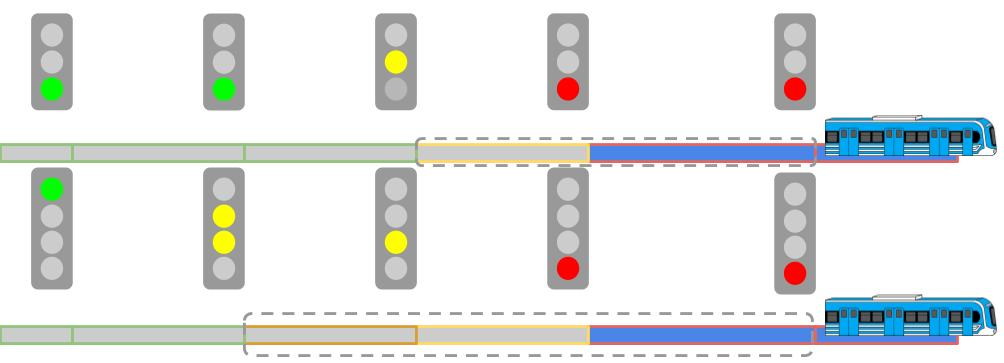
\includegraphics[scale=.4]{./Figures/Recubrimiento}
				\caption{Estado de los aspectos ferroviarios según la ubicación del tren.}
				\label{fig:Recubrimiento}
			\end{figure}
			\change{Incluir el tren recortado?}
			
			El sistema ferroviario sigue el principio de falla segura\footnote{fail-safe: Falla segura}. Es decir, si por alguna razón algo falla, el sistema adopta la condición mas restrictiva, mitigando la posibilidad de una situación peligrosa. Si la alimentación se corta o si el cableado sufre alguna falla, entonces el sistema asumirá que hay un tren y los semáforos se pondrán a rojo para que las formaciones cercanas detengan su marcha y las barreras de los pasos a nivel desciendan.		
			
		\subsection{Pasos a nivel}
		
			Un paso a nivel es una intersección entre una vía férrea y una calle o ruta peatonal, como se ilustra en la Figura \ref{fig:Paso_a_nivel}
			
			En ausencia de trenes, el sistema de control de la barrera del paso a nivel mantiene el brazo en alto para permitir la circulación de peatones y automóviles. Cuando un tren ocupa las secciones amarillas de la Figura \ref{fig:Paso_a_nivel} se desenergiza la barrera y comienza a descender el brazo por efecto de la gravedad. Cuando se ocupen las secciones azules de la Figura \ref{fig:Paso_a_nivel} entonces se accionará la alarma sonora para alertar a los peatones que deben permanecer en el laberinto contiguo a la vía, cuya función es forzar a los peatones a mirar a ambos lados antes de cruzar el paso a nivel.
			
			\begin{figure}[h!]
				\centering
				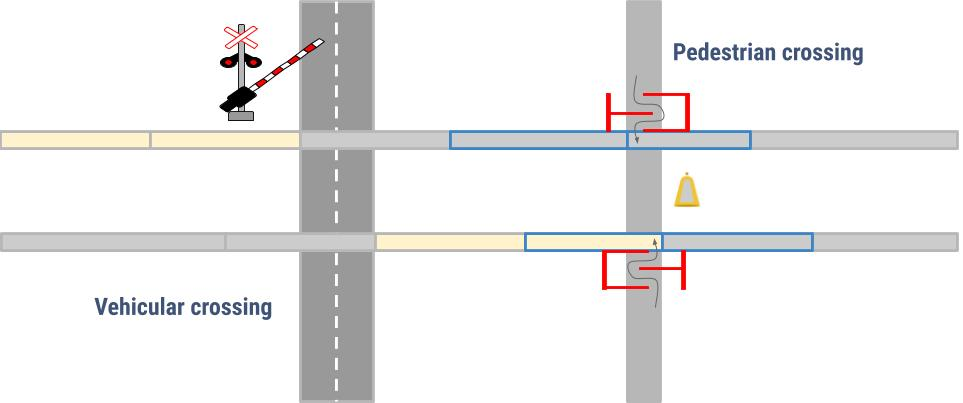
\includegraphics[scale=0.4]{./Figures/Paso a nivel}
				\caption{Pasos a nivel vehicular y peatonal sobre vía férrea.}
				\label{fig:Paso_a_nivel}
			\end{figure}
			\change{Rehacer figura}
			%\vspace{5cm}
			
			Solo cuando la barrera baja, el tren tiene permitido avanzar sobre el cruce, siendo el paso a nivel un sector de altísimo riesgo.
			
			Al desocuparse las las secciones amarillas, la barrera vuelve a energizarse y se sitúa en estado alto nuevamente, a la espera de otro tren para reiniciar el proceso descripto.
						
			Se debe destacar que el mismo proceso de descenso de la barrera ocurrirá si la misma se desenergiza por una falla eléctrica y/o pérdida de alimentación. Es decir, el sistema asumirá el estado mas seguro ante cualquiera de los mencionados fallos, siguiendo el principio de falla segura.
		
		\subsection{Máquina de cambios}
			
			Una máquina de cambios (Figura \ref{fig:Cambio}) posibilita el uso de rutas alternativas a la ruta principal para diversificar los itinerarios o ante cualquier incidente, permitiendo el paso de las formaciones de una vía a otro. Consiste en un mecanismo que mueve la aguja del cambio (riel móvil) hacia su respectiva contraaguja (riel fijo) hasta obtener un adecuado acoplamiento que permita la circulación de la formación.
			
			\begin{figure}[h!]
				\centering
				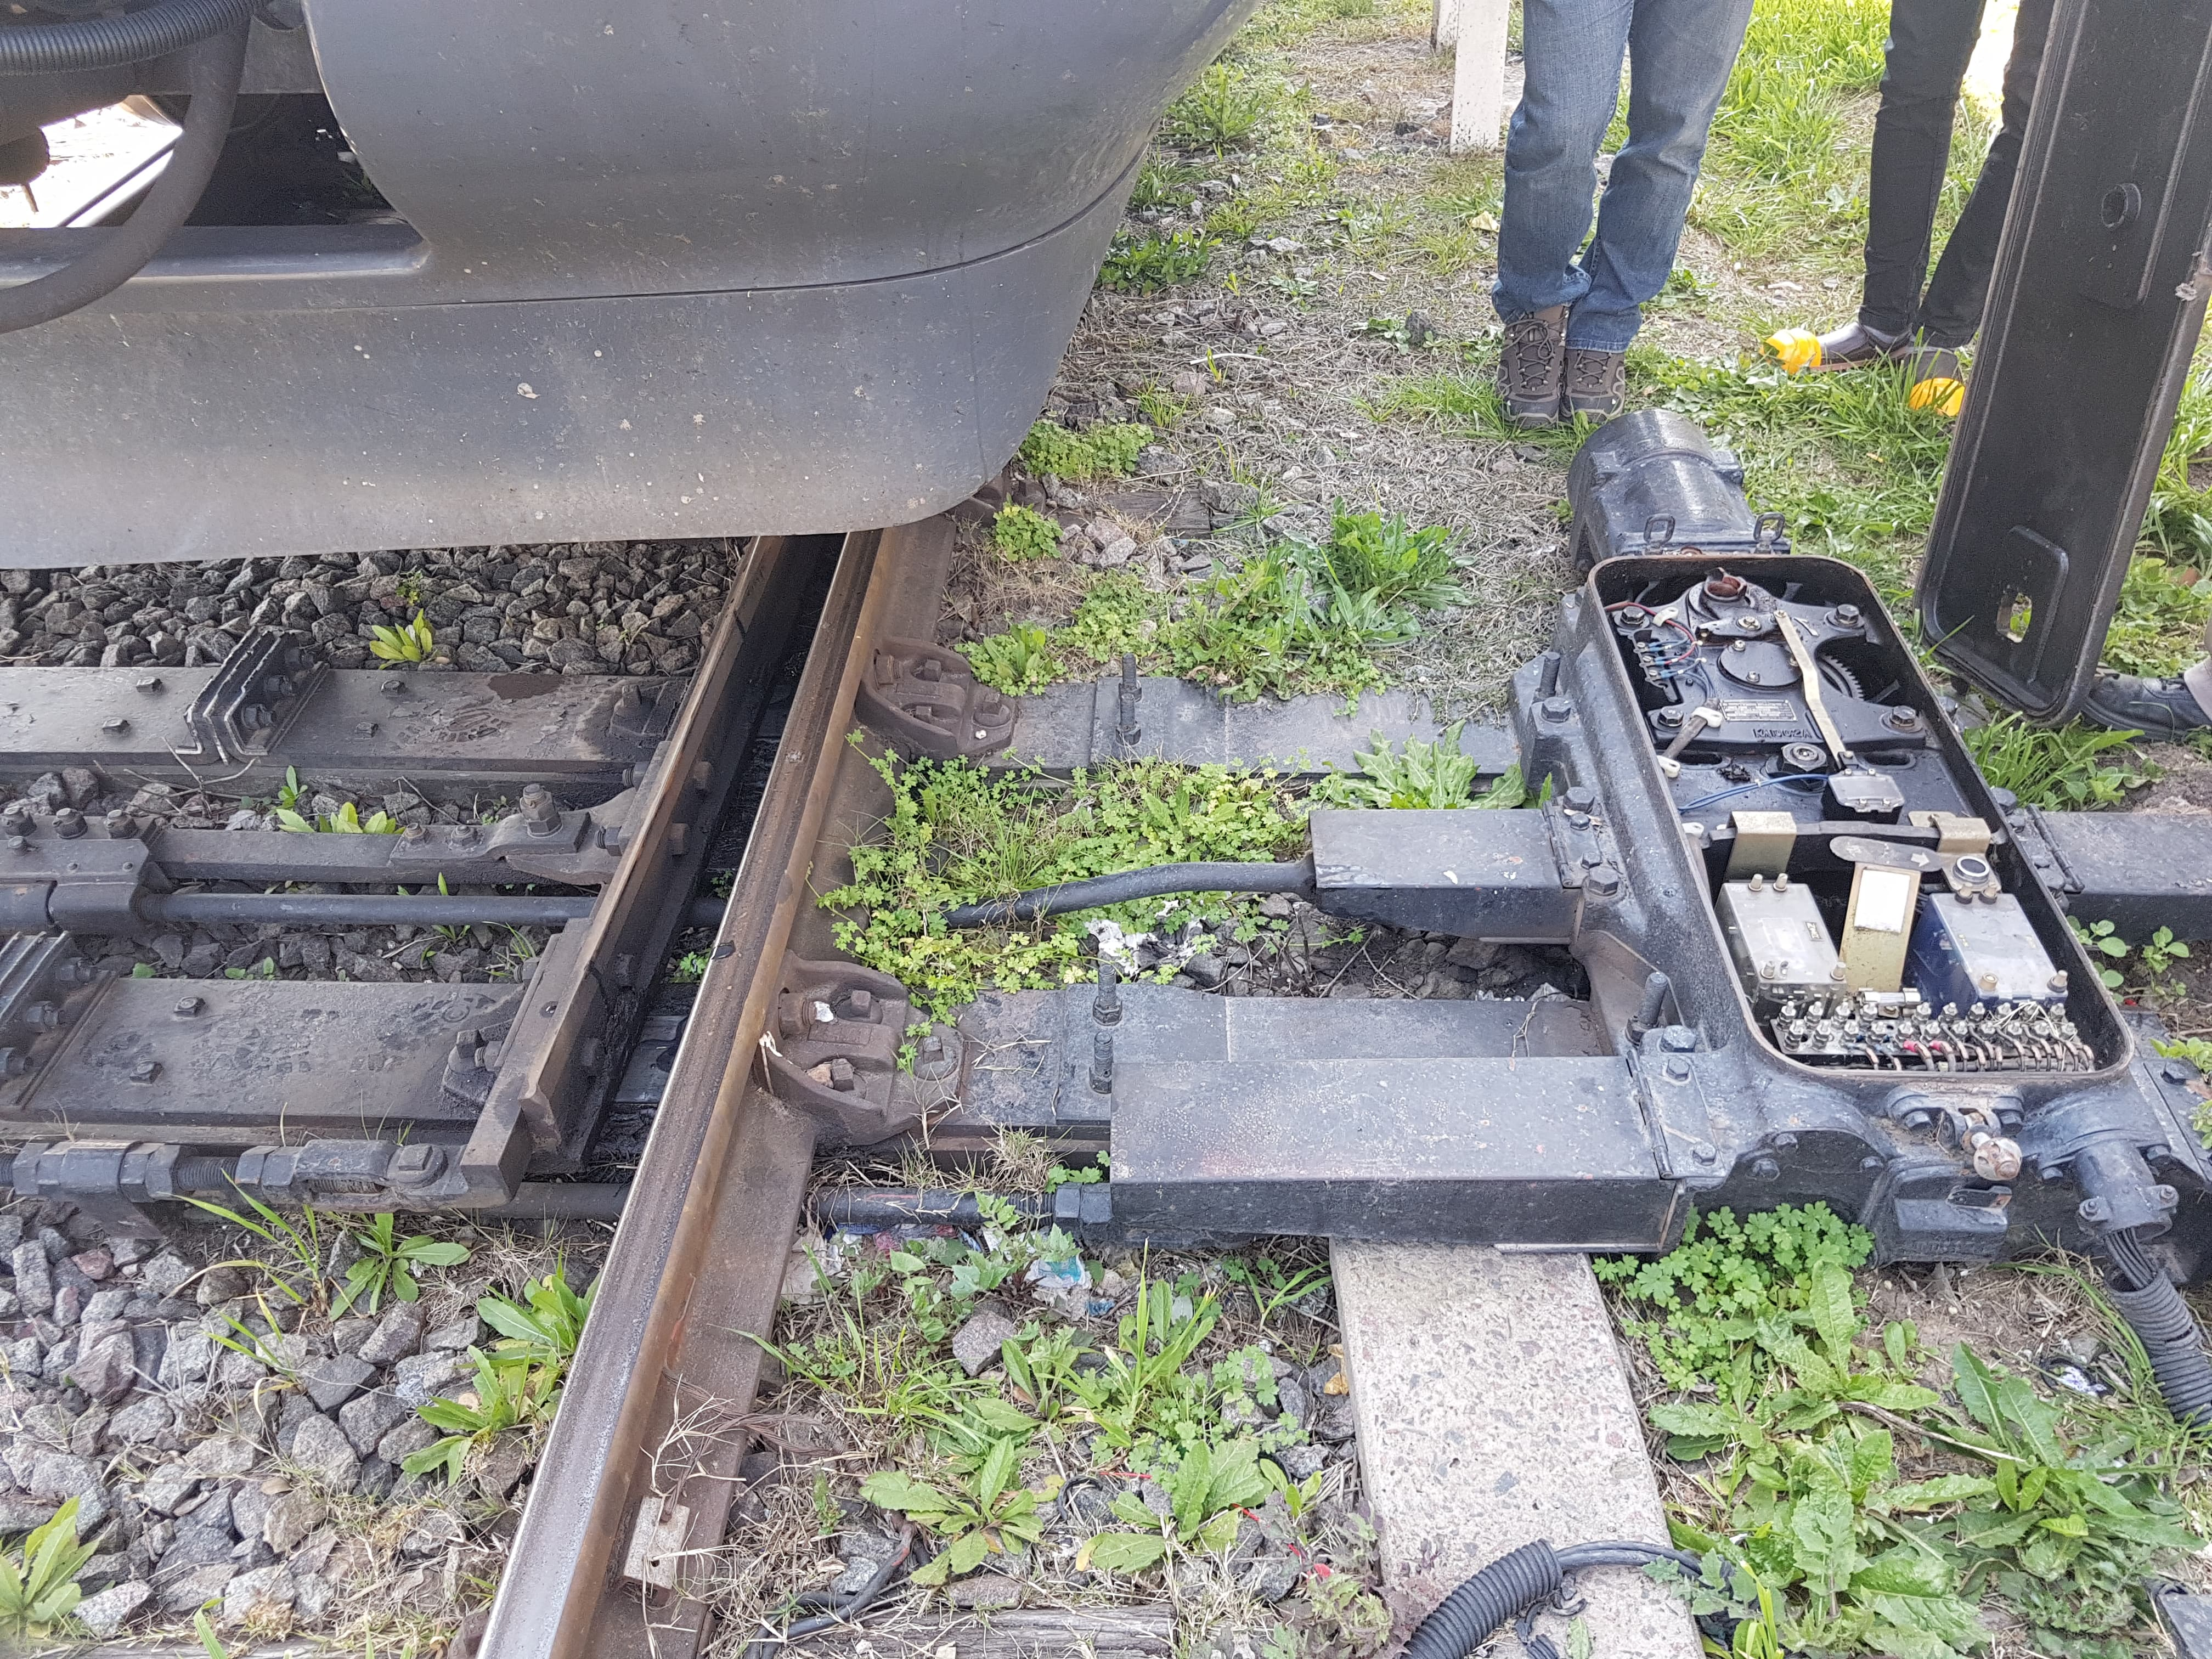
\includegraphics[scale=.06]{./Figures/Cambio}
				\caption{Máquina de cambios de Lavallol (Línea Roca).}
				\label{fig:Cambio}
			\end{figure} 
			
			\vspace{7cm}
			
			En la Figura \ref{fig:Cambios_2} se muestra el cambio de vía de la estación Matheu de la Línea Mitre. Se observa que según sea la posición del cambio el tren puede continuar en la misma vía o hacer el cambio a la otra vía.
			
			\begin{figure}[h!]
				\centering
				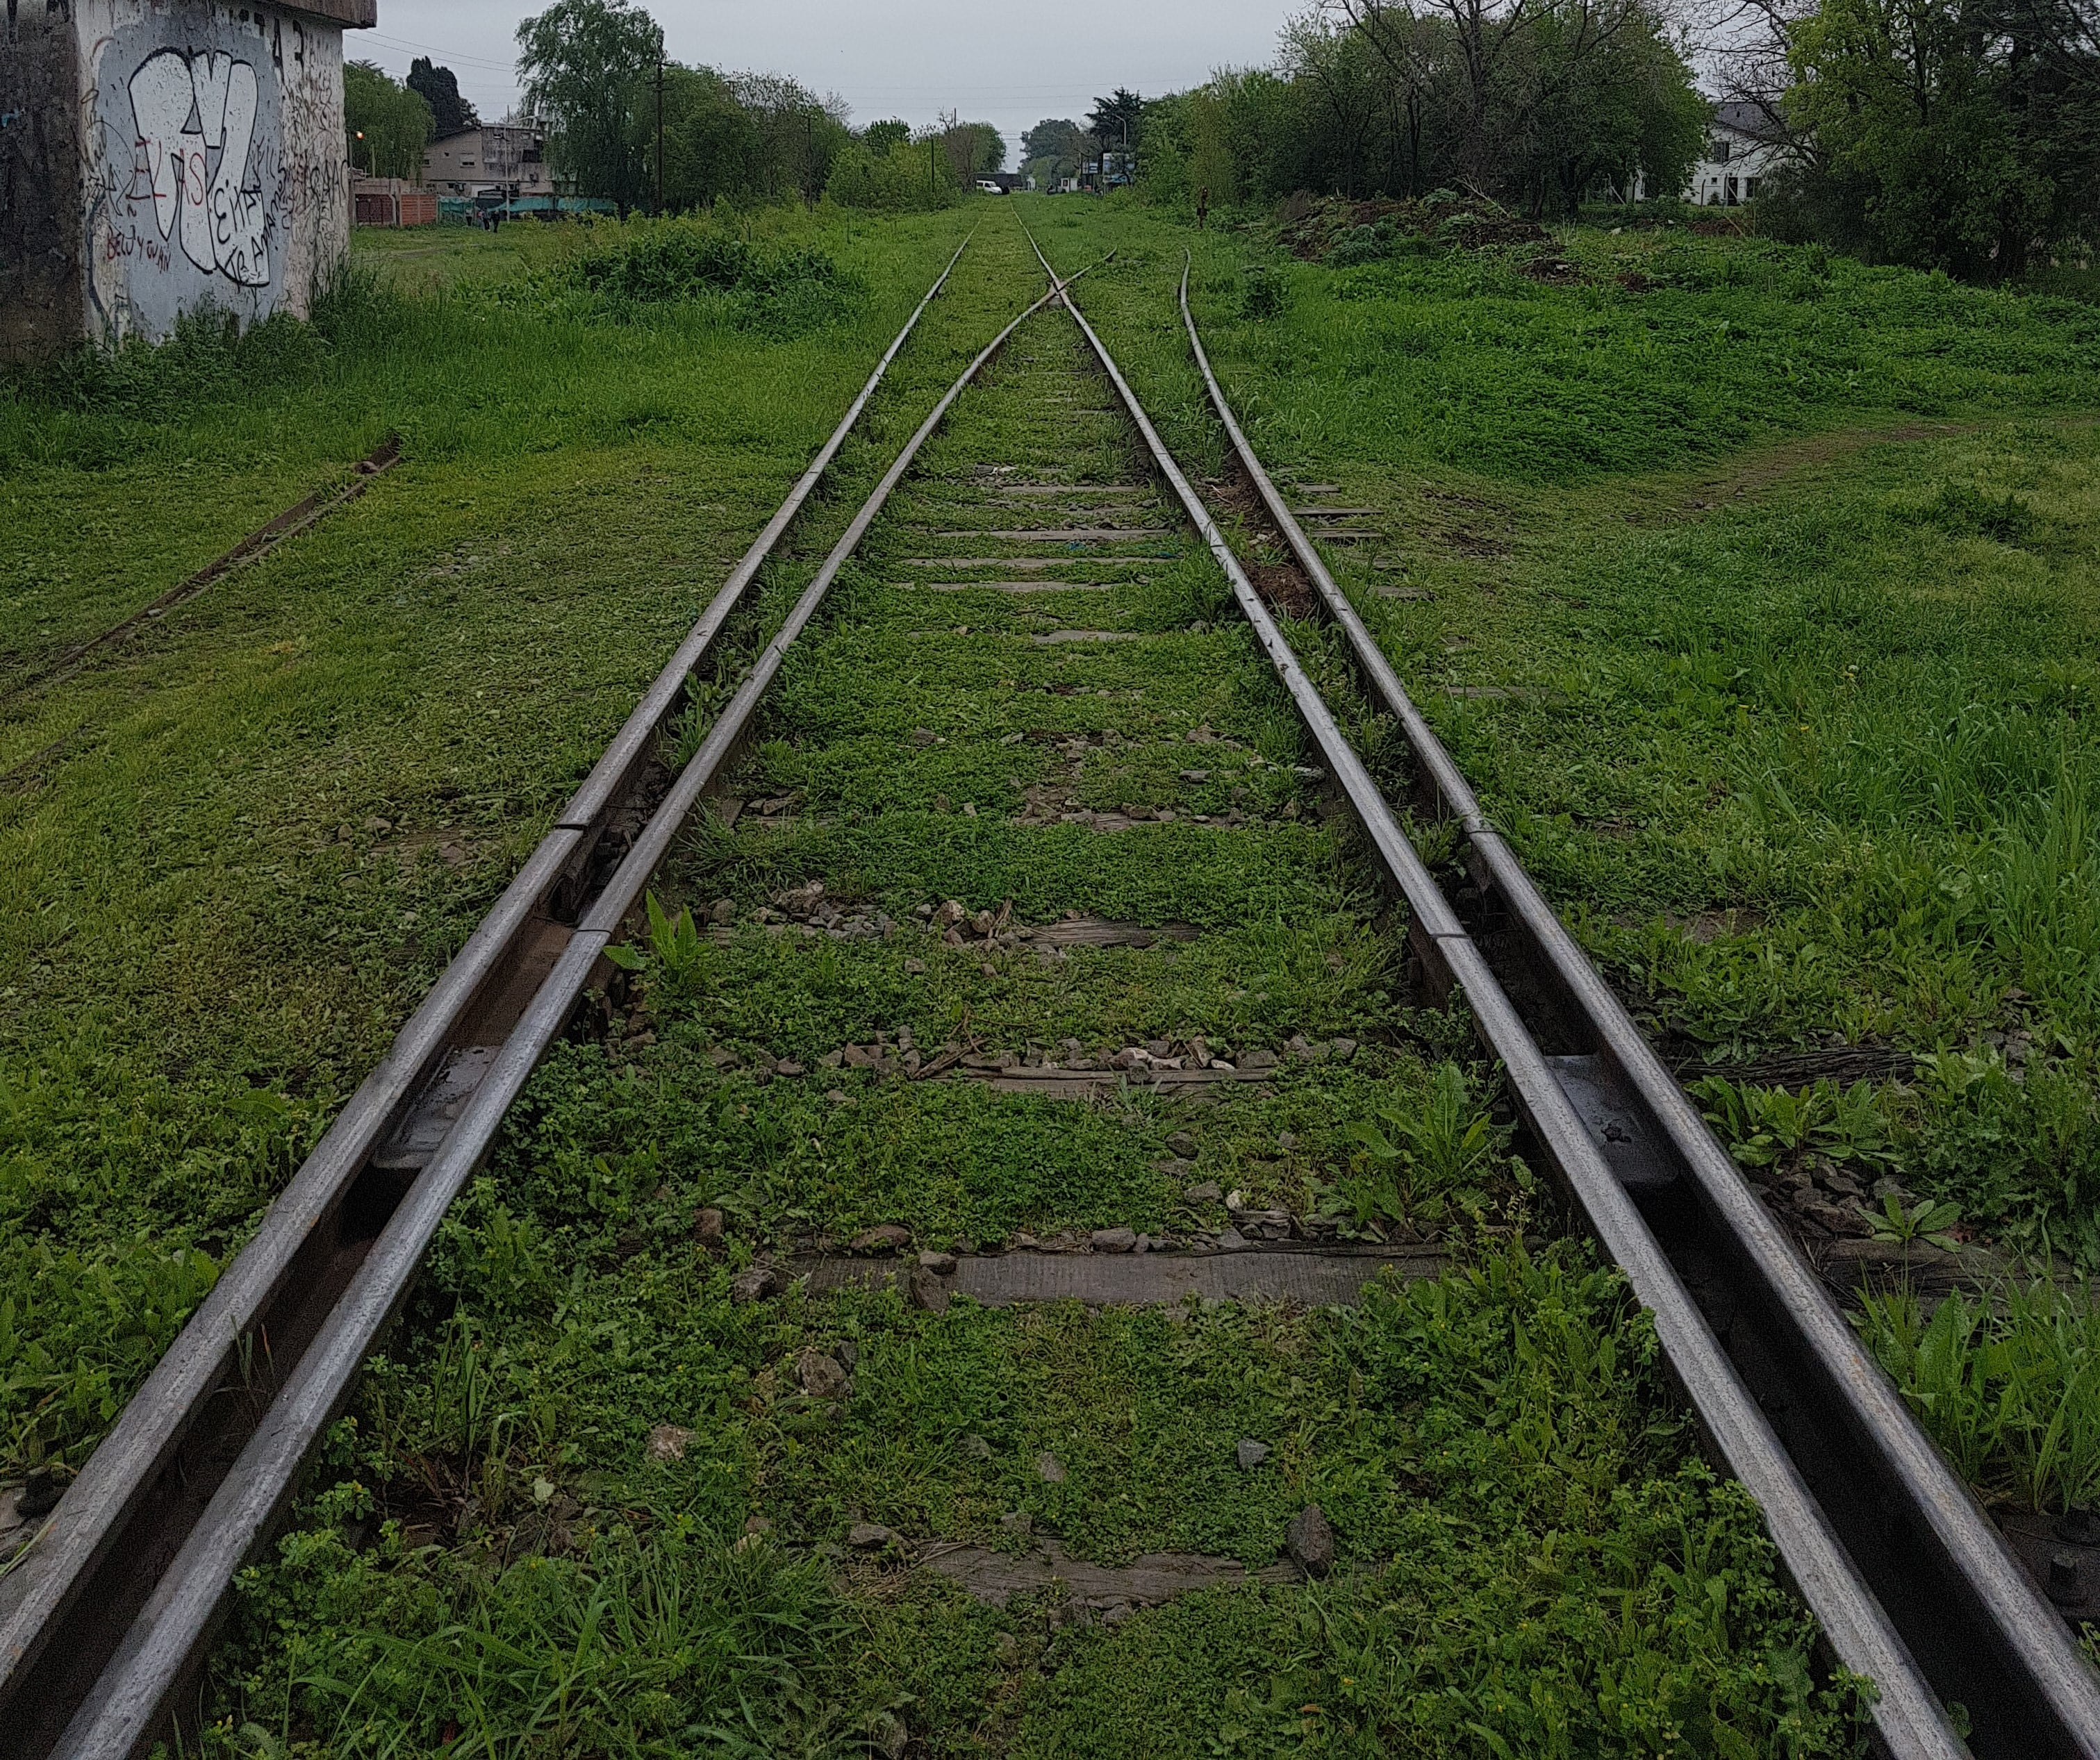
\includegraphics[scale=.1]{./Figures/Cambios_2}
				\caption{Cambio de vías de estación Matheu (Línea Mitre).}
				\label{fig:Cambios_2}
			\end{figure} 
		
			En la Figura \ref{fig:Cambios} se muestran las posiciones que puede adoptar el cambio. En la posición normal los trenes pueden circular de forma directa, en paralelo, por la vía principal en sentidos opuestos. En la posición reversa, en cambio, se permite el intercambio de trenes de una rama principal a otra en sentido opuesto o a una ramificación secundaria de la red.
			
			\begin{figure}[h!]
				\centering
				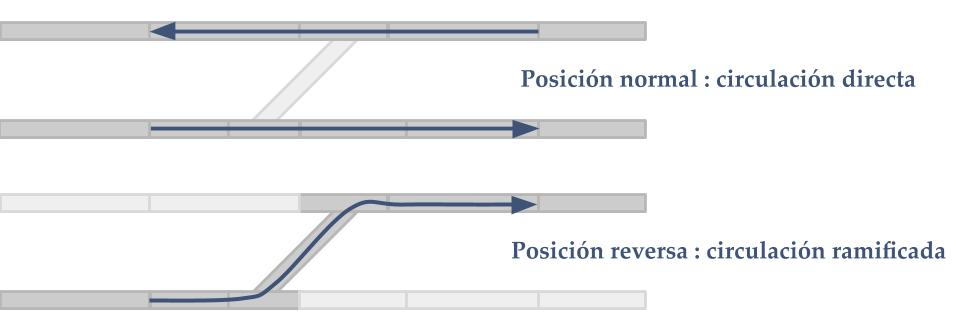
\includegraphics[scale=.45]{./Figures/Cambios}
				\caption{Posiciones normal e inversa del cambio.}
				\label{fig:Cambios}
			\end{figure} 
		
					
	\section{Sistema de enclavamientos}
	

		En la Figura \ref{fig:Bypass} se presenta, a modo de ejemplo, un sistema de cambios en una vía simple con \emph{bypass}. El mismo permite que una formación que transita hacia la estación B y una formación que lo hace hacia la estación A puedan cruzarse.
	
		\begin{figure}[h!]
			\centering
			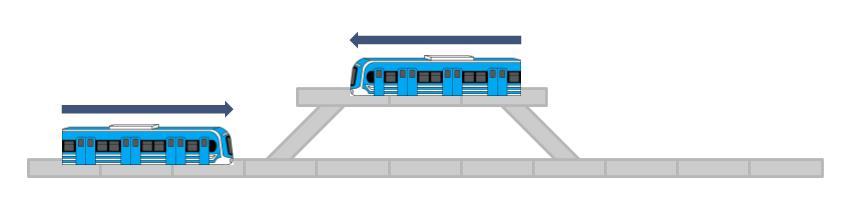
\includegraphics[scale=.45]{./Figures/Bypass_2}
			\caption{Vía simple con bypass}
			\label{fig:Bypass}
		\end{figure}
		\change{Rehacer figura}
		%\vspace{5cm}
				
		Este cruce mediante el uso del \emph{bypass} requiere un control seguro para evitar colisiones entre los trenes. Por ejemplo, si se aplica una configuración de las máquinas de cambios tal que dos formaciones en sentido opuesto sean conducidas ambas al bypass o sean conducidas ambas a la vía principal, entonces podría producirse una colisión entre los trenes. El sistema de enclavamiento impide que se produzcan estas configuraciones no seguras y controla los semáforos que habilitan o no los itinerarios de las formaciones.
	 
	 	Una falla en un enclavamiento puede ocasionar que se produzcan configuraciones no seguras y poner en peligro cientos de vidas humanas y generar costos considerables. Por lo tanto, en el diseño del sistema de enclavamiento se deben cumplir estrictos parámetros de fiabilidad, disponibilidad, mantenibilidad y seguridad (RAMS).
	 	
		 En Argentina la mayoría de los enclavamientos son mecánicos y tienen entre 40 y 100 años de antigüedad por lo que en muchos casos se ha agotado su vida útil y deben ser reemplazados. Otros en cambio, han estado en desuso por años y se necesita su reposición. Un ejemplo de esto es la ruta ferroviaria a la zona de Vaca Muerta, donde se requiere instalar sistemas de enclavamiento por cifras millonarias en dólares. Por esto, es importante contar con sistemas electrónicos de diseño y fabricación nacional.

		Adicionalmente, existen diferentes lugares donde aún resta instalar este tipo de sistemas, por lo que su implementación constituye una necesidad real para el desarrollo de la infraestructura ferroviaria de señalamiento en Argentina.		
	
	\section{Tipos de enclavamientos}
		
		A continuación se presentan distintas tecnologías de implementación de enclavamientos.
		
		\subsection{Enclavamientos mecánicos}
			
			A comienzos del siglo XX se implementaron los sistemas de enclavamientos mediante soluciones mecánicas. Utilizaban palancas como las que se visualizan en la Figura \ref{fig:Mecanico} para comandar los cambios de vías y semáforos.
	
			\begin{figure}[htbp!]
				\centering
				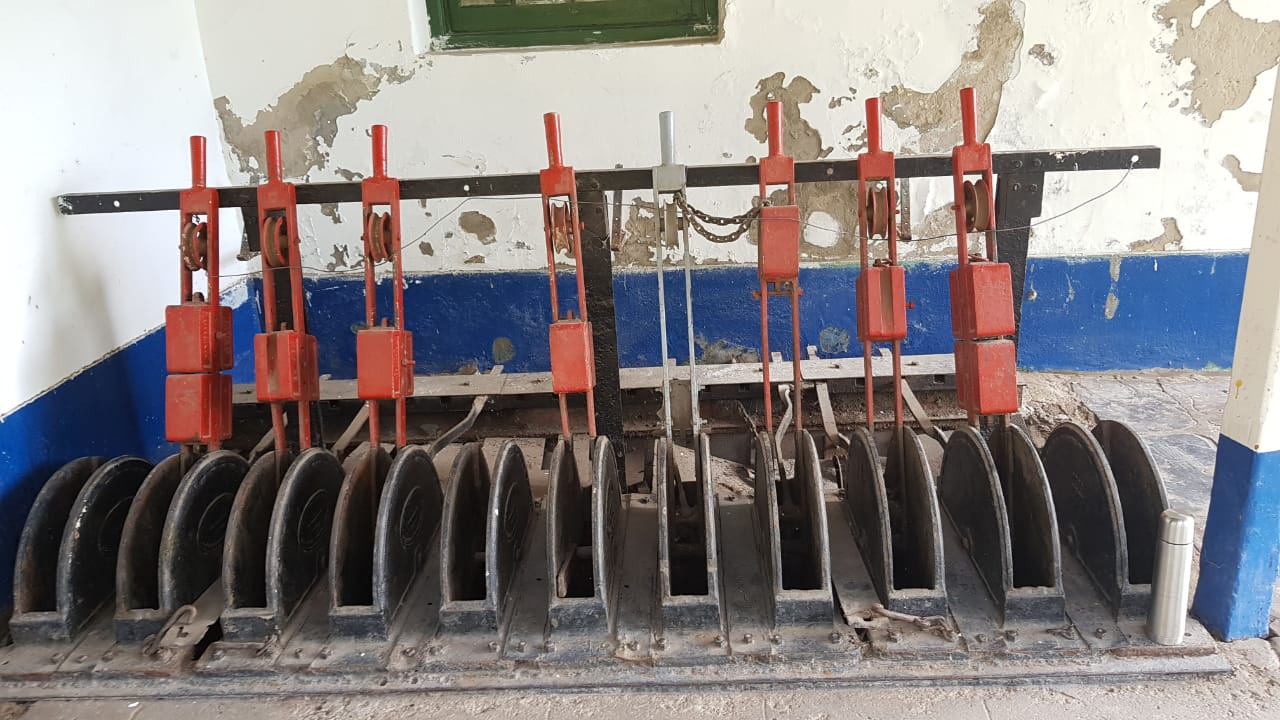
\includegraphics[scale=.3]{./Figures/Mecanico}
				\caption{Sistema mecánico de enclavamiento en la antigua estación de Chascomús, hoy convertida en museo.}
				\label{fig:Mecanico}
			\end{figure}

			Una vez que se constituye una configuración de posiciones de palancas que habilitan un trayecto, las mismas quedan 'enclavadas' mecánicamente. Es decir, la posición de las mismas se bloquea y no es físicamente posible cambiarla. A su vez a medida que se van moviendo ciertas palancas las demás palancas que pudieran representar situaciones no seguras quedan enclavadas, y sólo se pueden mover aquellas cuyo accionamiento representa una situación segura. De esa manera se garantiza que no se generarán configuraciones tales que las formaciones colisionen entre sí.
			
			Las tecnologías mas modernas heredaron el término 'enclavamiento', aún cuando ya no se tengan palancas enclavadas en posiciones fijas.
		
		\subsection{Enclavamientos electromecánicos}
			
			A mediados de siglo XX se desarrolló el sistema de enclavamiento electromecánico. Su funcionamiento se basa en relés (Figura \ref{fig:Reles}) y circuitos de vía, de forma tal de poder detectar la presencia de un tren y comandar tanto las señales como las barreras de los pasos a nivel.
	
			Se visitó un sistema de enclavamientos en la estación Lavallol (Línea Roca). La misma es una sala refrigerada, de gran tamaño, con varios bastidores que contienen cientos de relés. La Figura \ref{fig:Reles} corresponde al enclavamiento electromecánico de Lavallol.	
			
			\begin{figure}[htbp!]
				\centering
				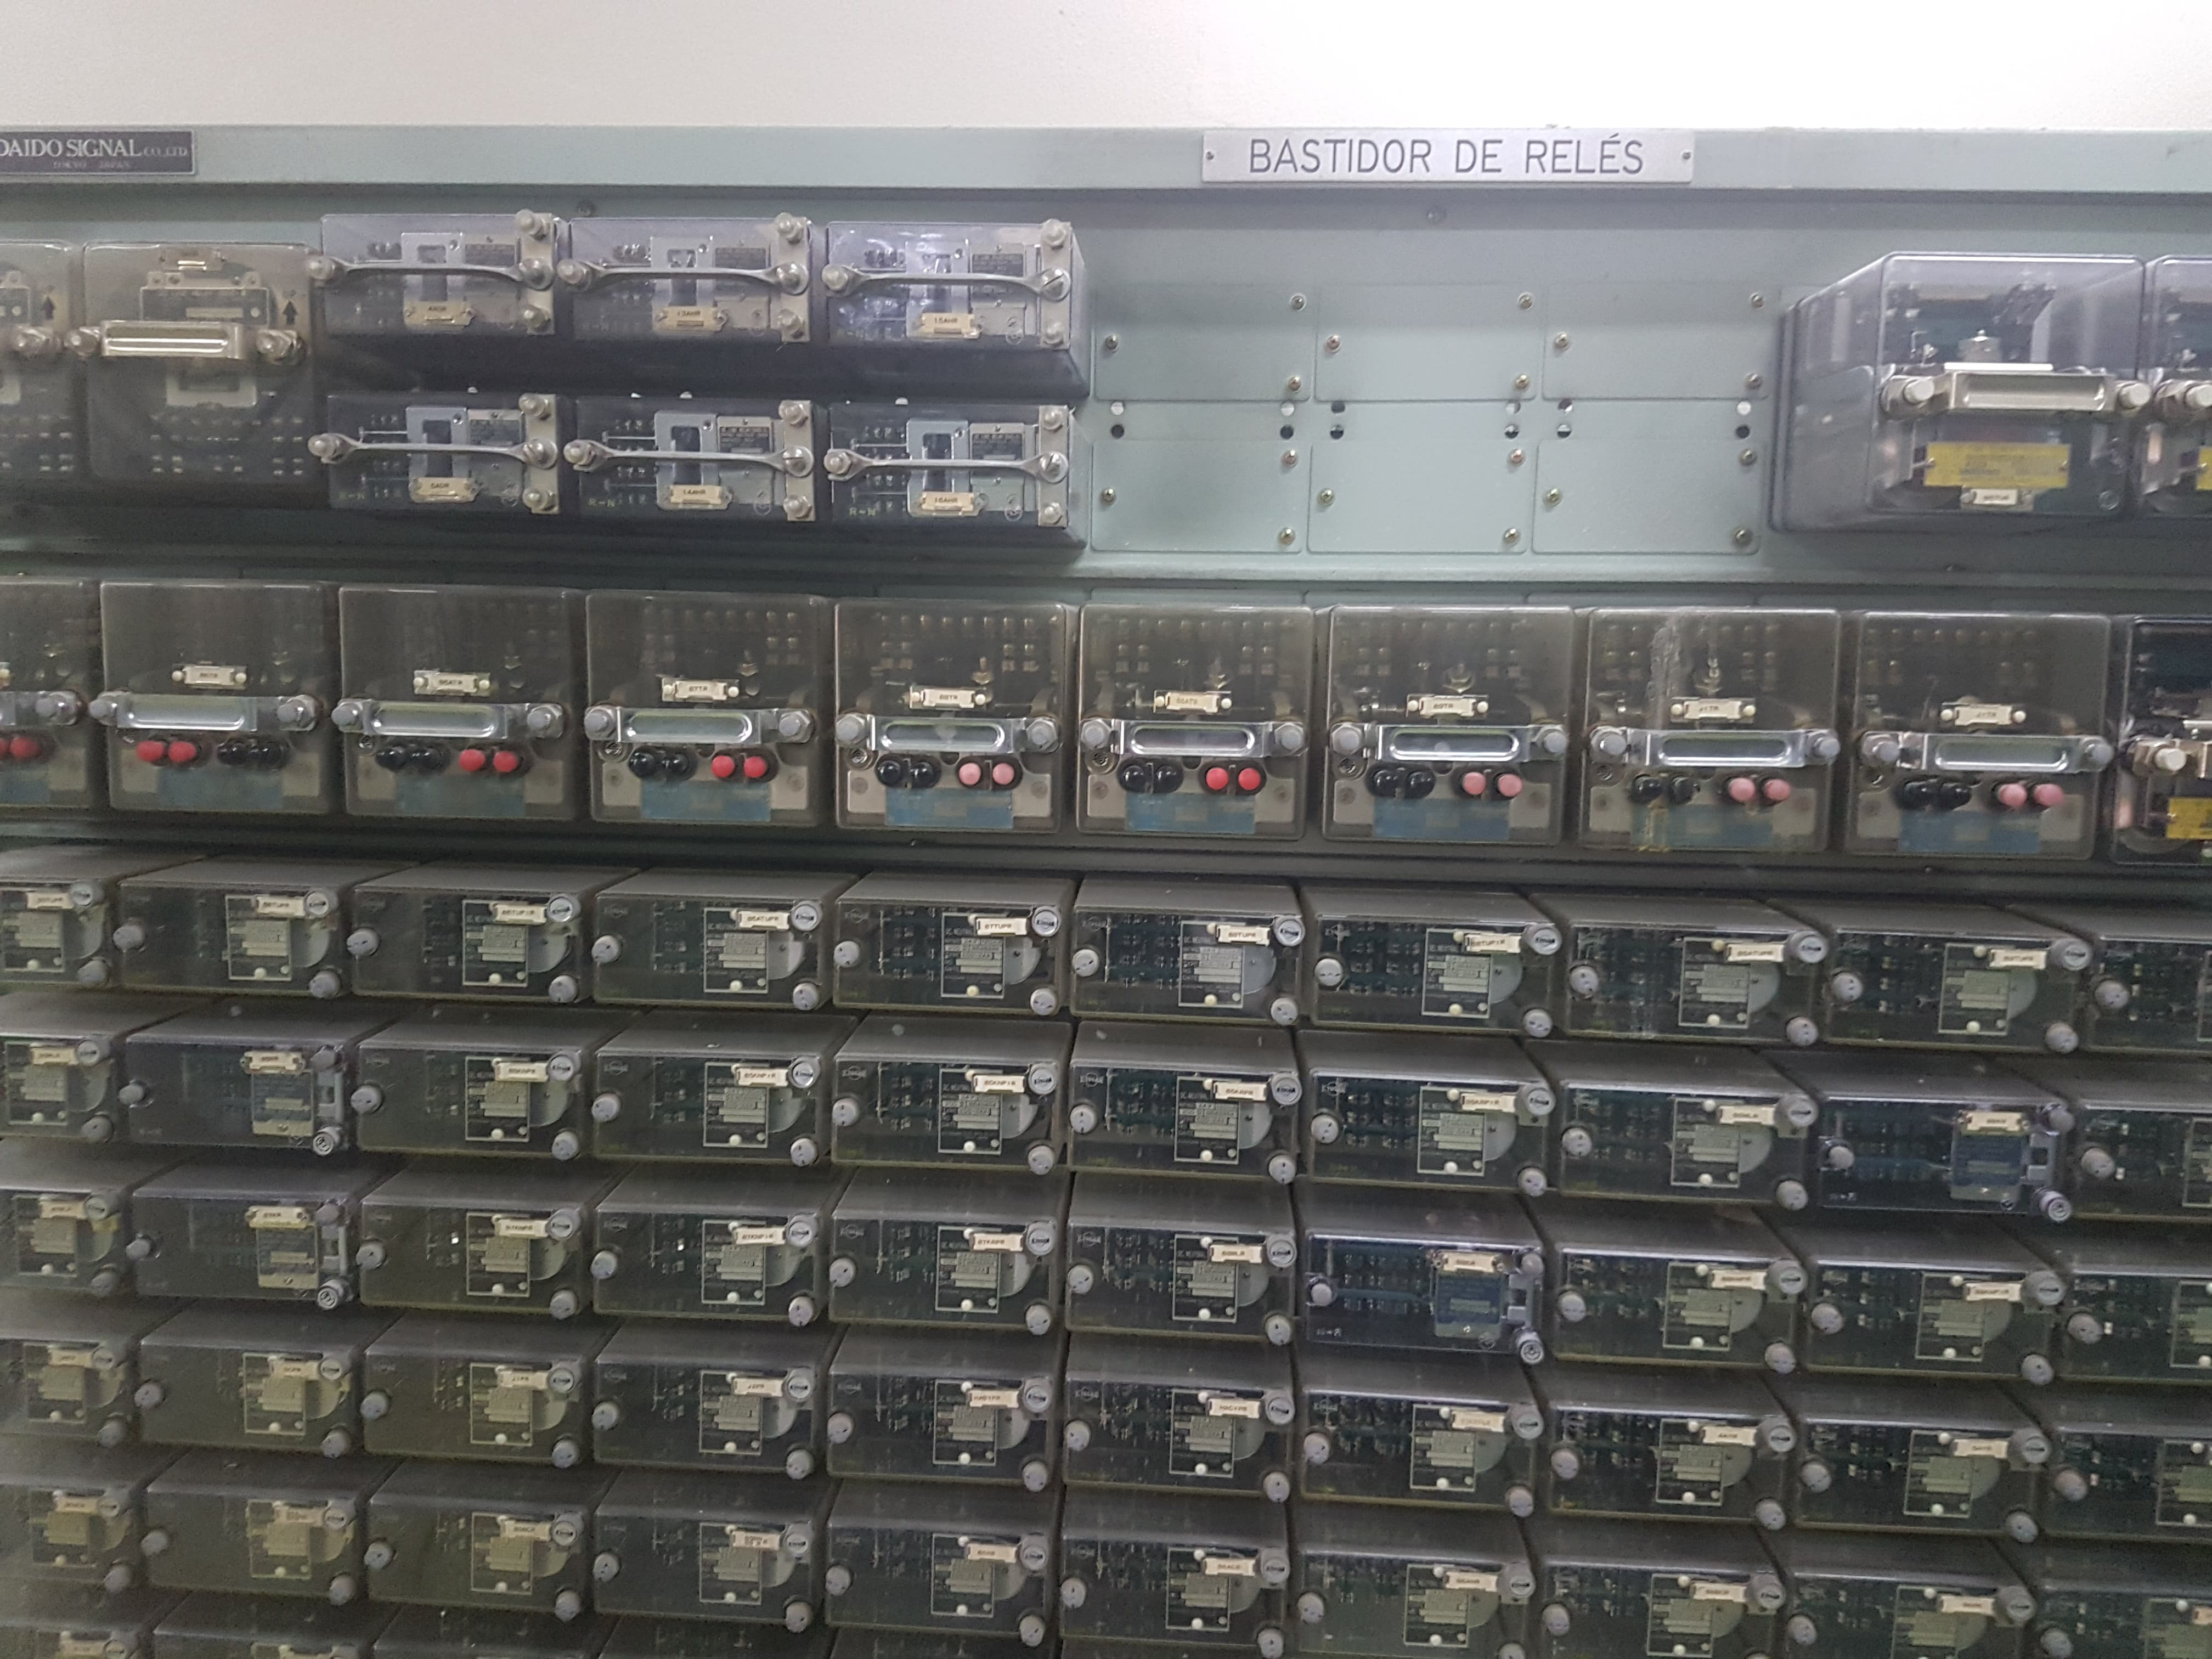
\includegraphics[scale=.08]{./Figures/Reles}
				\caption{Bastidor de relés de estación Lavallol.}
				\label{fig:Reles}
			\end{figure}
		
			%\vspace{5cm}
			
			Los sistemas de enclavamiento electromecánicos son comandados por un operario mediante un panel de control (Figura \ref{fig:Electromecanico}). El operario solicita al sistema de enclavamiento las rutas que el conductor ferroviario necesita para circular. El sistema permitirá solo la operación de cambio de vías seguras. En caso contrario, se tendrán las salidas 'enclavadas' y el sistema de enclavamiento impedirá mediante los semáforos el avance de la formación hasta que pueda realizarse el cambio en forma segura.
		
			\begin{figure}[h!]
				\centering
				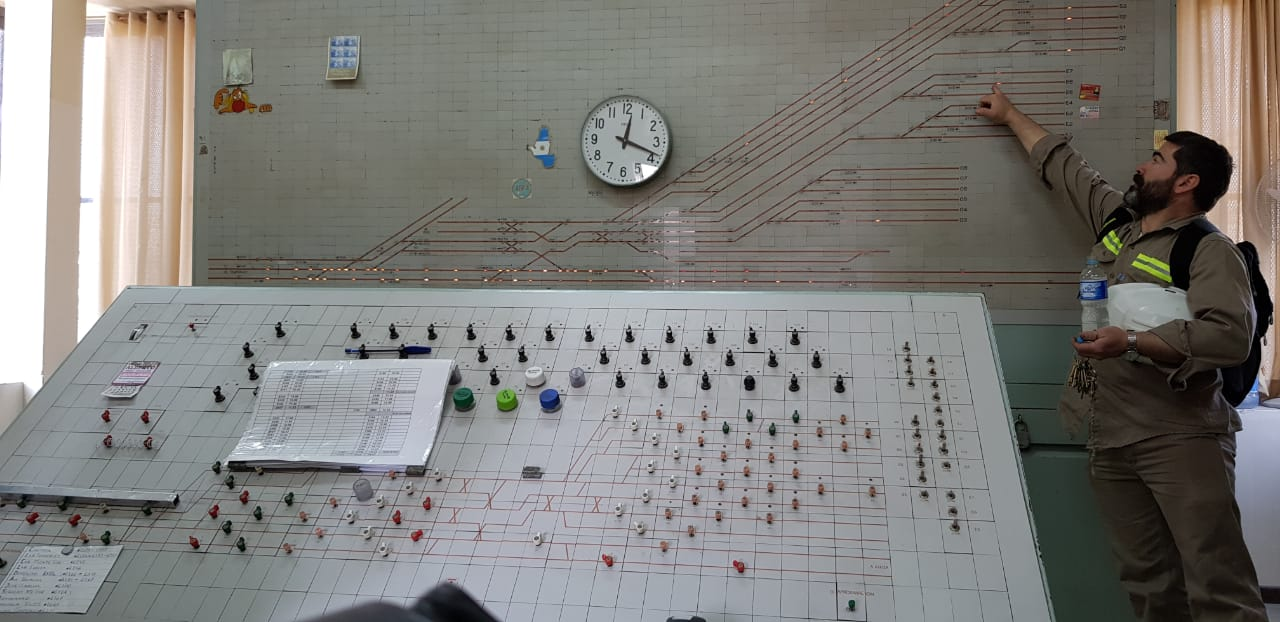
\includegraphics[scale=.27]{./Figures/Electromecanico}
				\caption{Panel de control enclavamientos - Central Lavallol.}
				\label{fig:Electromecanico}
			\end{figure}
		
			\vspace{5cm}
			
			%El sistema debe evitar colisiones en los trenes, pero no siempre se tiene toda la red con circuitos de vías. Por lo tanto es el operario el que debe recordar a que sectores envió tal o cual formación. Lo que implica una enorme responsabilidad que recae en el operario y el factor de error humano aumenta conforme el personal se encuentre mas cansado o distraído por alguna razón.
		
		\subsection{Enclavamientos electrónicos}
		\label{sec:Redundancia}	
			%La redundancia es obligatoria en sistemas electrónicos críticos para obtener un sistema tolerante a fallas, operando ante eventos no previstos u erróneos.
			
			El sistema de enclavamiento moderno es electrónico y debe incluir redundancia de hardware para lograr niveles RAMS adecuados. Pueden utilizarse, por ejemplo, estrategias de \emph{2 en 2} o sistemas de votación \emph{2 de 3}  como se ve en la Figura \ref{fig:Redundancia} para tener siempre una salida sin importar los fallos que puedan producirse\citep{REDUNDANCIA}. La diversidad de plataformas de hardware (representados en diferente color en la Figura \ref{fig:Redundancia}), por ejemplo utilizando diferentes proveedores de un mismo sistema o plataforma, es otra técnica muy utilizada.
			
			\begin{figure}[h]
				\centering
				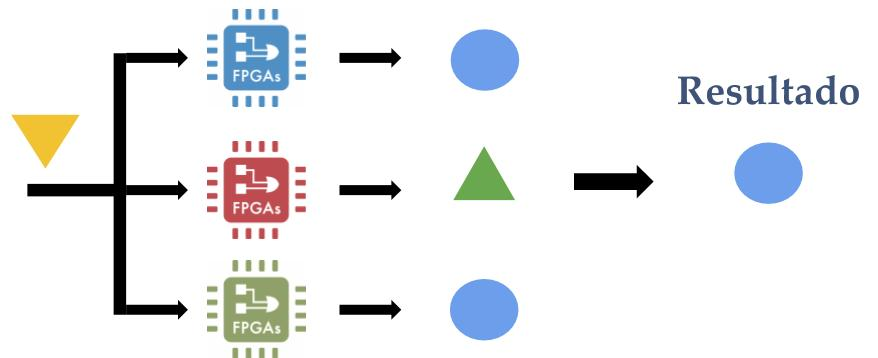
\includegraphics[scale=.45]{./Figures/Redundancia}
				\caption{Redundancia por votación 2 de 3.}
				\label{fig:Redundancia}
			\end{figure}
			
			En este trabajo se implementó un sistema de enclavamiento electrónico, como se explicará en el Capítulo \ref{Chapter3}.
	 
	 		%\vspace{5cm}
	 		
%	\section{Tabla de enclavamientos}
%	\label{Tabla_enclavamientos}
%	\label{sec:Semi}	
%		La forma de diseñar y presentar los enclavamientos es mediante tablas de enclavamiento. La Figura \ref{fig:Matheu_a} presenta la tabla correspondiente a la estación Matheu de la Línea Mitre.
%	
%		\begin{figure}[htbp!]
%			\centering
%			%\includegraphics[scale=.4]{./Figures/Matheu_a}
%			\caption{Tabla de enclavamientos mecánicos (Matheu-Mitre).}
%			\label{fig:Matheu_a}
%		\end{figure}
%		
%		La tabla define en que posiciones se enclavan las palancas de la segunda columna, respecto de las condiciones de la columna 'normal' e 'invertida'.
%		
%		Por ejemplo, en el caso de la palanca 1, que corresponde a la señal de distancia 2 y 3, si las palancas 2 y 3 se encuentran en posición invertida, entonces la palanca 1 se enclavará en invertida sin posibilidad de pasarla a normal hasta que las otras dos palancas reviertan su estado.
%			
%		En este trabajo se utiliza una forma alternativa de representar las tablas de enclavamiento, que se introduce a continuación, mediante un ejemplo en base a la Figura \ref{fig:Esquema_vacio}.		
%		
%		\begin{figure}[htbp!]
%			\centering
%			%\includegraphics[scale=.3]{./Figures/Tabla_vacia}
%			\caption{Esquema de ejemplo en el que las señales no se han asignado.}
%			\label{fig:Esquema_vacio}
%		\end{figure}
%		
%		\vspace{5cm}
%		
%		Se supone una topología de vías dobles con un cambio de vías entre ambas para realizar maniobras, dos pasos peatonales con campanilla (paso a nivel 1 y 3) y un paso a nivel vehicular con barrera automática (paso a nivel 2). 
%		
%		Además se presentan los semáforos de tres aspectos correspondientemente numerados de forma creciente en el sentido de circulación marcado para cada trayecto (impares para la vía ascendente y pares de la descendente). Se ilustran además, los semáforos de dos aspectos (10 y 11) para las maniobras de cambio de vías.
%		
%		Para comenzar el razonamiento, todo el señalamiento se muestra apagado (gris) ya que se busca determinar en qué aspecto debe estar cada señal. Supóngase que una formación ocupa el circuito de vía 8, detenido antes del semáforo 6 y se dispone a completar el trayecto descendente hacia la sección 6 de la vía.%, correspondiente a la estación. %Cabe destacar que el cambio de vía en este caso se toma en reversa, por lo que se denomina una 'maniobra de talón'.
%		
%		%Si nos encontramos en el modo semiautomático, el operario debe solicitar al sistema de enclavamiento cada ruta que desee que la formación recorra. Una ruta siempre se define de un semáforo al semáforo inmediatamente consecutivo. Por lo tanto mientras la ruta no esté aprobada los semáforos deben estar en aspecto rojo y como la aprobación requiere la presencia de una formación ocupando el circuito de vía inicial de la misma, se concluye que la vía ascendente tendrá todos los semáforos en rojo en ausencia de formación alguna.
%		
%		Ya que la formación usará la vía principal, los semáforos 10 y 11 correspondientes al cambio de vías también estarán a rojo, al igual que los semáforos 2 y 8 que no involucran a la ruta a solicitar. La ruta en cuestión se definirá entre los semáforos 6 (inicial) y el 4 (final). Para comenzar el trayecto la formación necesita permiso para acceder a los tramos de vías siguientes, para lo cual el semáforo 6 deberá estar en aspecto verde. Para finalizar el trayecto se necesita que el semáforo 4 se encuentre en rojo. Por seguridad se pusieron a rojo el semáforo 8 (para evitar colisiones de formaciones que vengan antes de la formación de ejemplo) y el semáforo 2 (por si la formación no llega a frenar ante el semáforo 4).
%		
%		El paso a nivel número 3 debería estar a peligro desde que la formación ocupo el circuito de vía 10, el número 2 debería tener su barrera baja por la misma razón y el número 1 estará a peligro tan pronto la formación ocupe el circuito de vía 6b. Por lo tanto los tres pasos a nivel se encuentran a peligro y no deberán permitir el cruce ni de vehículos ni de peatones mientras la ruta esté en ejecución. Durante todo el trayecto también se deberá garantizar que la máquina de cambios se encuentre en posición 'normal'. De esta forma se tiene la configuración que se muestra en la Figura \ref{fig:Esquema_lleno}.
%		
%		\begin{figure}[htbp!]
%			\centering
%			%\includegraphics[scale=.3]{./Figures/Tabla_llena}
%			\caption{Esquema de ejemplo en el que las señales se han asignado.}
%			\label{fig:Esquema_lleno}
%		\end{figure}
%		
%		La Tabla \ref{tab:Ejemplo_semi} representa la situación descripta, siendo:
%		
%		\begin{table}[htbp!]
%			\centering
%			\caption[Modelo de Tabla de enclavamientos semiautomáticos]{Modelo de Tabla de enclavamientos semiautomáticos}
%			\resizebox{\textwidth}{!}{  
%			\begin{tabular}{c|cccccc|ccccc|cccc|cc|c|ccc}    
%				\toprule
%				& \multicolumn{6}{c|}{Circuitos de vía (DES)} & \multicolumn{5}{c|}{Semáforos ASC} & \multicolumn{4}{c|}{Semáforos DES} & \multicolumn{2}{c|}{Cambio} & M & \multicolumn{3}{c}{PaN} \\
%				\textbf{Rutas} 	 & 2 & 4 & 6a & 6b & 8 & 10 & 1 & 3 & 5 & 7 & 9 & 2 & 4 & 6 & 8 & 10 & 11 & - & 1 & 2 & 3  \\
%				\midrule
%				$\text{Ruta}$ &O&O&O&O&X&O&R&R&R&R&R&R&R&V&R&R&R&N&B&B&B\\ 
%				%\bottomrule
%				\hline
%			\end{tabular}
%			}
%			\label{tab:Ejemplo_semi}
%		\end{table}
%		
%		\begin{itemize}
%			\item O: Circuito de vía que debe permanecer libre.
%			\item X: Circuito de vía que se encuentra ocupado por una formación.
%			\item R: Semáforo rojo.
%			\item A: Semáforo amarillo.
%			\item V: Semáforo verde.
%			\item -: \emph{Don't care}, no es relevante.
%			\item N: Máquina de cambios en posición normal.
%			\item R: Máquina de cambios en posición reversa.
%			\item A: Barrera alta.
%			\item B: Barrera baja.
%		\end{itemize}								
%		
%		Repitiendo el razonamiento se pueden generar las demás filas de la tabla para cualquier ruta entre dos semáforos. Solo se puede tener un tren en cada vía a la vez: uno para la vía ascendente y otro para la vía descendente.
%		
%%		En el caso del modo automático la construcción de la tabla es muy similar, pero cambia el criterio para los semáforos.
%%		
%%		Por otro lado, en el modo automático los semáforos por defecto se encuentran en verde y cada tren que ocupa la vía genera hacia atrás una estela de protección denominada doble recubrimiento[REF] a peligro como puede verse en la Figura \ref{fig:Doble}.
%%		
%%		\begin{figure}[htbp!]
%%			\centering
%%			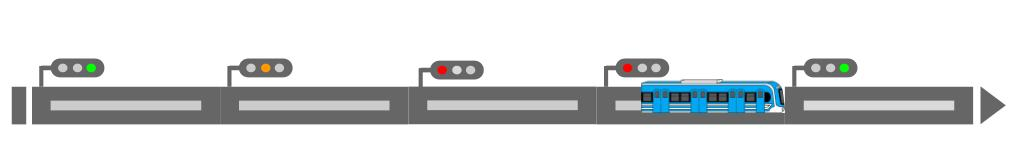
\includegraphics[scale=.33]{./Figures/Doble}
%%			\caption{Doble recubrimiento a peligro}
%%			\label{fig:Doble}
%%		\end{figure}
%%				
%%		Dicho recubrimiento consiste en dos semáforos a rojo (semáforo 7 y 9) para proteger el tramo que ocupa la formación y el anterior (circuitos de vía 11 y 9), además de un semáforo amarillo de precaución (semáforo 5) para avisar a la formación anterior que la próxima señal será roja y debe disminuir su marcha.					
%%		
%%		En esta modalidad no se pueden realizar cambios de vías, por lo que la máquina de cambios estará en posición 'normal' y los semáforos de cambios 10 y 11 estarán en rojo. Además todos los pasos a nivel estarán a peligro menos el paso a nivel número 1, que al estar alejado de la formación que sigue avanzando en sentido ascendente, dejará de sonar su campanilla.
%%		
%%		La Tabla \ref{tab:Ejemplo_auto} presenta el ejemplo anterior pero para un sistema automático con una formación ocupando el circuito de vía 4.
%%		
%%		\begin{table}[htbp!]
%%			\centering
%%			\caption[Modelo de Tabla de enclavamientos semiautomáticos]{Modelo de Tabla de enclavamientos semiautomáticos}
%%			\resizebox{\textwidth}{!}{  
%%			\begin{tabular}{c|cccccc|ccccc|cccc|cc|c|ccc}    
%%				\toprule
%%				& \multicolumn{6}{c|}{Circuitos de vía(ASC)} & \multicolumn{5}{c|}{Semáforos ASC} & \multicolumn{4}{c|}{Semáforos DES} & \multicolumn{2}{c|}{Cambio} & M & \multicolumn{3}{c}{PaN} \\
%%				\textbf{Rutas} 	 & 1 & 3 & 5 & 7 & 9 & 11 & 1 & 3 & 5 & 7 & 9 & 2 & 4 & 6 & 8 & 10 & 11 &  & 1 & 2 & 3  \\
%%				\midrule
%%				$\text{Ruta}$ &-&-&-&O&O&X&V&V&A&R&R&V&V&V&V&R&R&N&A&B&B\\ 
%%				%\bottomrule
%%				\hline
%%			\end{tabular}
%%			}
%%			\label{tab:Ejemplo_auto}
%%		\end{table}
%%	
%%		Los circuitos de vía 1,3 y5 figuran como \emph{don't care} porque queda fuera del doble recubrimiento y podría ser ocupado por otra formación. Además el semáforo para acceder a dicho tramo se establece en verde, lo que permite el acceso.
%		
	\section{Objetivos}
	
		El objetivo de este proyecto fue el diseño, implementación y realización de pruebas funcionales de un prototipo de sistema electrónico de enclavamiento, sobre un kit de desarrollo de FPGA. 
		
		Se procura además estudiar las tecnologías para implementar metodologías orientadas a mejorar los niveles RAMS del sistema, de acuerdo al estado del arte en sistemas ferroviarios altamente críticos. 
		
		Teniendo la experiencia acumulada del trabajo realizado en la Especialización de Sistemas Embebidos, se puso especial énfasis en la automatización del proceso, para poder satisfacer las necesidades de cualquiera sea la estación o zona elegida. 

%		Para lo cual se definieron los siguientes requerimientos funcionales:
%		
%		\begin{itemize}
%			\item Cantidad de entradas: alrededor de 40
%			\item Tipo de entrada: contactos secos
%			\item Clase de entradas: ocupación de vía, señalamiento, estado de la máquina de cambios o posición de barreras del paso a nivel.
%			\item Tiempo máximo entre cambios: 1 minuto
%			\item Topología: vía doble con estación, cruce y tres pasos a nivel
%			\item Distancia mínima entre formaciones: doble recubrimiento
%			\item Tiempo mínimo para recorrer el tramo:
%			\item Tiempo máximo para recorrer el tramo:
%			\item Cantidad de trenes circulando en simultáneo: hasta 2 en modo semiautomático y hasta cuatro en modo automático.
%			\item Cantidad de coches por formación: 6
%		\end{itemize}

	
%----------------------------------------------------------------------------------------






